\documentclass[12pt]{article}
\usepackage{enumitem}
\usepackage{hyperref}
\usepackage{polyglossia}
\setdefaultlanguage{french}
\usepackage{fontspec}
\usepackage{graphicx}
\usepackage{amsmath, amssymb}
\usepackage{color}
\emergencystretch=2.5em

\title{IFT3295 - TP1}
\author{Assemblage de séquences}
\date{25 septembre 2026}
 

\begin{document}

\maketitle
\section*{Évaluation}
\begin{itemize}
	\item  Ce TP est à faire en équipe de deux (pas d’équipe de trois).
	\item Vous devez le rendre au plus tard le
	      vendredi 9 octobre 2026 avant la démo ($\leq13h29$).
	\item Deux fichiers à remettre: le code Python pour le programme demandé (un fichier
	      zip si plus d'un fichier)
	      et un pdf pour les autres questions.
	\item Utiliser Studium pour la remise du TP. Une version papier des questions écrites est aussi
	      correcte.
	\item \textbf{Vous devez utiliser le squelette de code fourni avec le TP}
	      ({\it main.py}, {\it overlap.py}, {\it assembly.py}, {\it utils.py},
	      {\it run.sh})~: complétez les fonctions marquées
	      \texttt{NotImplementedError~\#TODO} en conservant les signatures et
	      les annotations de types fournies, ainsi que l'interface en ligne de
	      commande de {\it main.py}. Le script {\it run.sh} exécute le
	      pipeline complet (matrice, graphe, fragment).
	\item \textbf{Il est formellement interdit d'utiliser des librairies
	      externes pour faire l'alignement ou l'assemblage de séquences}~:
	      vous devez implémenter vous-même les algorithmes. Pour le graphe,
	      vous pouvez utiliser la librairie NetworkX afin de construire votre
	      graphe et le convertir en format dot.
	\item Votre code doit être bien lisible et compréhensible (bonne
	      indentation, noms de variables et de fonctions représentatifs, commentaires,
	      etc.).
\end{itemize}


\section*{Mise en situation}

Vous commencez un stage dans le laboratoire du Dr Osborn. Ce dernier
étudie activement un nouveau virus et a récemment identifié une protéine
humaine X impliquée dans la synthèse de protéines virales. Il décide donc
d'étudier cette nouvelle protéine pour mieux comprendre son rôle dans les
infections virales. Pour ce faire, Dr Osborn séquence la région génomique
contenant le gène de la protéine X . La technologie qu'il utilise produit des
petits fragments chevauchant appelés {\it reads} qui recouvrent la région
d'intérêt,
dans un seul sens de lecture (voir figure suivante).

\begin{figure}[h]
	\centering
	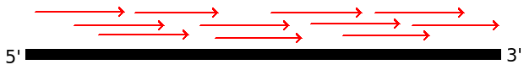
\includegraphics[width=9cm]{reads.png}
\end{figure}

Le Dr Osborn requiert votre
assistance pour assembler tous les reads afin d'obtenir la séquence nucléotidique
de la région génomique.

\section*{Chevauchement de séquences (25pts)}

Veuillez considérer les pondérations suivantes :
\begin{itemize}
	\item "match" : +4
	\item "mismatch" : -4
	\item "indel" (insertion ou suppression) : -8
\end{itemize}

Pour assembler les reads, vous devez considérer pour chaque paire (ordonnée) de séquence
${X_i, X_j}$ , le meilleur alignement tel que le chevauchement (tel illustré
sur la
figure suivante) entre $X_i$ et $X_j$ soit de score maximal.


\begin{figure}[h]
	\centering
	
\includegraphics[width=7cm]{chevauchement.png}
\end{figure}

Afin de développer un algorithme pour le problème du chevauchement
maximal entre deux séquences, répondez aux questions suivantes :
\begin{enumerate}


	\item  Quelle est la différence entre un tel alignement et l'alignement global?
	\item  Quelles doivent être les valeurs de la première ligne ( $V (0,j) \forall
		      j$ )? et
	      celles de la première colonne ( $V (i, 0) \forall i$ ) de la table de
	      programmation
	      dynamique V ? Justifiez votre réponse.
	\item  Quelles sont les équations de récurrence à utiliser pour remplir la table
	      de programmation dynamique?
	\item  Comment peut-on retrouver l'alignement avec le meilleur chevauchement à
	      partir de la table de programmation dynamique? Vous devez
	      décrire la procédure entière pour retrouver l'alignement.
	\item  Implémenter l' algorithme de programmation dynamique de tel sorte qu'il fonctionne en temps $O(|X_i||X_j|)$ pour trouver l'alignement maximisant le
	      chevauchement entre deux séquences et son score en fonction des coûts
	      donnés plus haut. Vous devez remettre un code qui retourne pour une
	      paire (ordonnée) de séquences : le score, l'alignement correspondant et la longueur du
	      chevauchement. Votre programme doit prendre comme
	      argument un fichier en format FASTQ contenant les deux séquences. Une description du format FASTQ est disponible
	      sur
	      \href{https://fr.wikipedia.org/wiki/FASTQ#Exemple_type}{wikipédia}.

\end{enumerate}



\section*{Assemblage de fragments (40pts)}

En vous servant de votre algorithme précédent, vous pouvez procéder à l'assemblage des séquences. À cet effet,
vous
disposez d'un fichier {\it reads.fq} qui contient les séquences et identifiants
de 20 reads en format FASTQ.

\begin{enumerate}


	\item  Pour chaque paire (ordonnée) de reads ${R_i, R_j}$, calculer le score de
	      l'alignement
	      correspondant au chevauchement maximal entre $R_i$ et $R_j$. On vous
	      demande une matrice 20x20. Notez que le score de chevauchement de ${R_i, R_j}$ est différent de celui de ${R_j, R_i}$ et donc que la matrice n'est pas symétrique.
	      La diagonale de la matrice est nulle.
	\item  En déduire le graphe orienté de chevauchement $G = (V, E)$ où $V$ désigne
	      l'ensemble des reads. Il existe une arête $e_{ij} = (R_i, R_j) \in E$
	      entre $R_i$ et $R_j$ s'il existe un chevauchement entre un suffixe de $R_i$
	      et un préfixe de $R_j$.
	      Pour vous aider à répondre aux questions suivantes vous pouvez utiliser
	      \href{https://www.graphviz.org/pdf/dotguide.pdf}{graphviz dot} ou n'importe
	      quel autre outil de visualisation de graphes.
	      \begin{enumerate}
		      \item  Afin de ne considérer que les chevauchements pertinents, filtrez les
		            alignements par leurs scores, en considérant un seuil minimum de
		            80 en dessous duquel les chevauchements sont ignorés. Quel effet
		            a ce seuil sur le graphe résultant?


		      \item  Afin d'assembler les reads, vous devez vous servir du graphe de
		            chevauchement. Cependant, ce dernier contient plusieurs arêtes
		            "inutiles" et peut donc être simplifié. Vous utiliserez le principe de
		            la réduction transitive (illustrée sur la figure suivante) qui enlève
		            les arêtes entre deux noeuds, tant qu'il existe encore un chemin
		            simple reliant ces deux noeuds. On vous demande l'ordre des reads
		            dans le graphe réduit, ainsi que la longueur du chevauchement
		            entre deux reads consécutifs.\\
		            Note:
		            Lorsque vous réduisez le graphe, si vous avez des cycles
		            contenant seulement deux noeuds, conservez uniquement l'arête de
		            plus grand score et supprimez l'autre.
		            \begin{figure}[h]
			            \centering
			            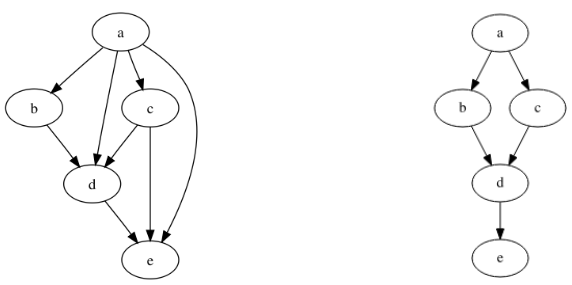
\includegraphics[width=9cm]{graphes.png}
		            \end{figure}

		      \item  Déduire la séquence du fragment génomique séquencé et sa longueur.
	      \end{enumerate}
\end{enumerate}
\newpage
\section*{Recherche d'introns et Blast (20pts)}

Grâce à votre aide, le Dr Osborn a finalement obtenu la séquence géno-
mique désirée ({\it sequence.fasta}). À partir d'une autre expérience, il a
réussi à
identifier la séquence protéique du gène X ({\it geneX.fasta}). Il désire
maintenant
identifier la séquence de l'ARNm du gène ainsi que ses introns.
\begin{enumerate}


	\item  Identifier la position de la protéine X au sein de la région génomique.
	      Pour ce faire traduisez d'abord la séquence nucléotidique de ({\it
			      sequence.fasta}) dans les trois différents cadres de lecture, en considérant
	      qu'il s'agit du
	      brin codant. Utilisez le code génétique standard (disponible ici ==>
	      \href{https://www.ncbi.nlm.nih.gov/Taxonomy/Utils/wprintgc.cgi?chapter=tgencodes#SG1}{table génétique}).
	      Veuillez noter que les nucléotides et les acides aminés
	      sont toujours représentés par un seul caractère dans les séquences et
	      que le signal de terminaison de la traduction (stop) peut être représenté
	      par une étoile (*). Répondez aux questions suivantes:
	      \begin{enumerate}


		      \item  Dans quel cadre de lecture se trouve le codon start de la séquence
		            protéique?
		      \item  Décrivez un algorithme de programmation dynamique (conditions initiales, relations des récurrence, chemin à suivre dans la table pour retrouver l'alignement optimal) permettant de retrouver le gène de la protéine en minimisant les introns. En raison d'erreur de séquençage, on autorisera des mismatchs dans les exons, mais pas de indels. Vous pouvez supposer que tous les exons sont dans le même cadre de lecture.
	      \end{enumerate}
	\item  En vous servant de l'outil
	      \href{
		      https://blast.ncbi.nlm.nih.gov/Blast.cgi?PROGRAM=blastp&PAGE_TYPE=BlastSearch&LI
		      NK_LOC=blasthome}{Blastp} et/ou de
	      \href{https://www.uniprot.org/blast/}{uniprot} , identifiez le nom
	      de la protéine X ainsi que sa fonction.
\end{enumerate}

\newpage
\section*{Repliement d'ARNs (15pts)}

Pour les questions suivantes,  étant donné une séquence d'ARN $S$, on veut retrouver le repliement en une ou plusieurs tiges-boucles de $S$ qui maximise le nombre d'appariement de bases. Notez qu'une tige-boucle peut contenir des nucléotides non-appariés et que seuls les appariements (A-U et G-C) sont considérés.
\begin{enumerate}
	\setcounter{enumi}{6}
	\item
	      Considérez la séquence d'ARN ci-dessous avec ses paires de bases inférées. Dessinez un repliement en 2D qui illustre les sous-structures principales de la molécule.
	      \begin{figure}[h]
		      \centering
		      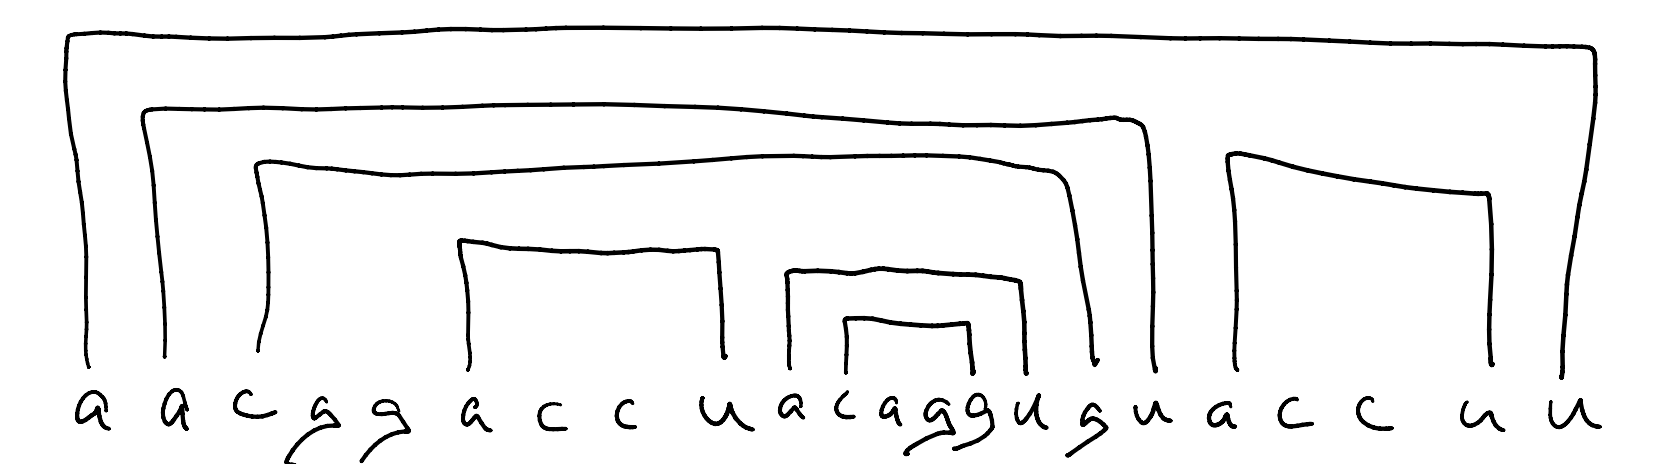
\includegraphics[scale=0.30]{Exercice6.png}
	      \end{figure}
\end{enumerate}

\begin{enumerate}
	\setcounter{enumi}{7}
	\item {\bf Bonus :}
	      Suposons que l'on veuille maximiser le nombre d'empilements, c'est-à-dire le nombre d'appariements (i,j) tels que (i+1,j-1) sont aussi appariés. Décrivez un algorithme de programmation dynamique (conditions initiales, relations des récurrence, chemin à suivre dans la table pour retrouver l'alignement optimal) fonctionnant en temps temps $O(n^3)$ qui permet de retrouver un repliement en une ou plusieurs tige-boucles maximisant le nombre d'empilements.

\end{enumerate}
\end{document}
